

\chapter{Mediated Perception Approach}
	\section{Perception}
		\subsection{Lane detection \& tracking}
		\subsubsection{Distortion Correction}
    		\begin{figure}[htbp]
            \centerline{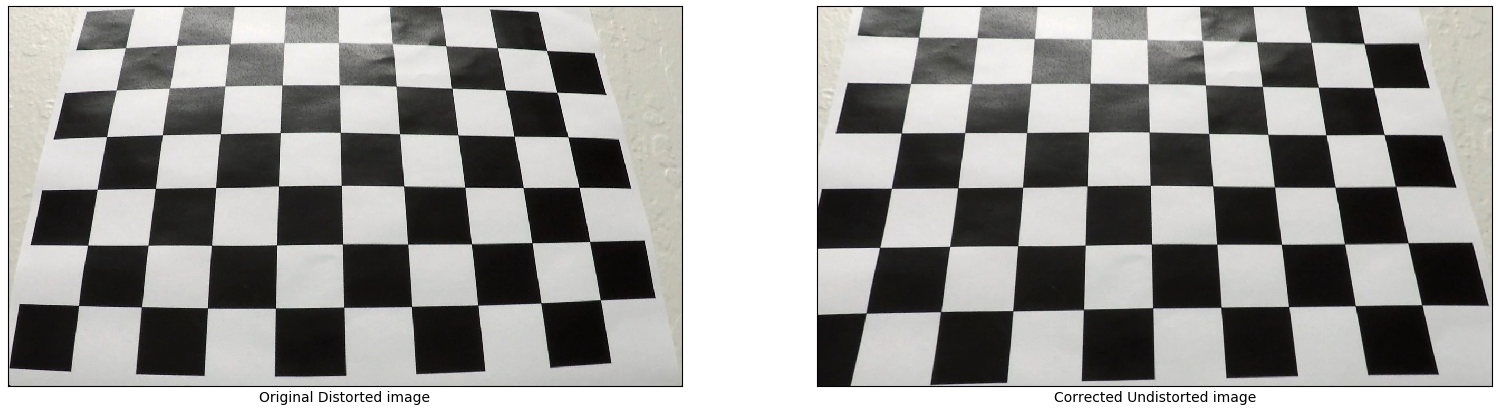
\includegraphics[width=\linewidth]{Figures/undist_chess.png}}
            \caption{Chess board image undistortion}
            \end{figure}
    		Lenses are used to focus an image on a camera sensor, which often causes light rays to bend at the edges of these lenses. This results in a distortion at the edges of images. Accordingly, lines and objects appear with a different curvature than their actual nature. This is referred to as radial distortion, which is the most common type of distortion.
    		
    		Tangential distortion is another common form of distortion. This occurs as a result of the camera’s lens being misaligned. When the lens is not perfectly parallel to the imaging plane, on which the camera sensor is mounted, an image look tilted so that some objects appear farther away or closer than they actually are.
    		
            \begin{figure}[H]
            \centerline{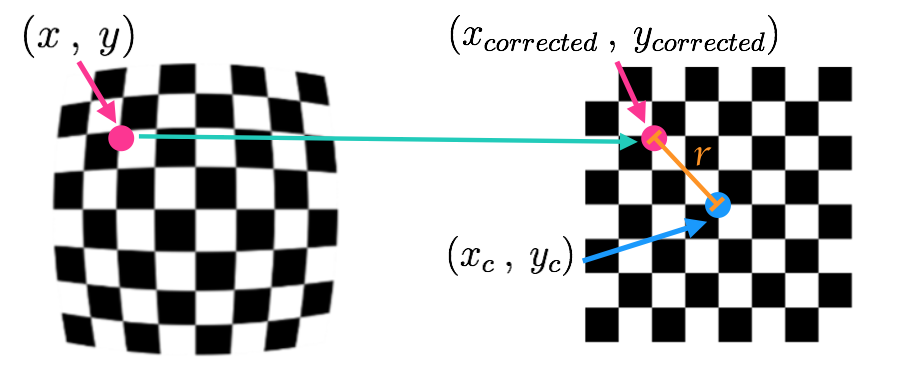
\includegraphics[width=\linewidth]{Figures/undistort.png}}
            \caption{Chess board image undistortion illustration}
            \end{figure}
            
    		Three coefficients needed to correct for radial distortion: \(k1, k2, and k3\) using the following correction formula
    		\begin{equation}
    		    x_{distorted} = x_{ideal} (1 + k_1 r^2 + k_2 r^4 + k_3 r^6)
    		\end{equation}
    		\begin{equation}
    		y_{distorted} = y_{ideal} (1 + k_1 r^2 + k_2 r^4 + k_3 r^6)
    		\end{equation}


    
    
        	I start by preparing "object points", which will be the (x, y, z) coordinates of the chessboard corners in the world. Here I am assuming the chessboard is fixed on the (x, y) plane at z=0, such that the object points are the same for each calibration image. Thus, objp is just a replicated array of coordinates, and objpoints will be appended with a copy of it every time I successfully detect all chessboard corners in a test image. imgpoints will be appended with the (x, y) pixel position of each of the corners in the image plane with each successful chessboard detection.
            
            I then used the output objpoints and imgpoints to compute the camera calibration and distortion coefficients using the cv2.calibrateCamera() function. I applied this distortion correction to the test image using the cv2.undistort() function and obtained this result:
    
            

            
            \begin{figure}[htbp]
            \centerline{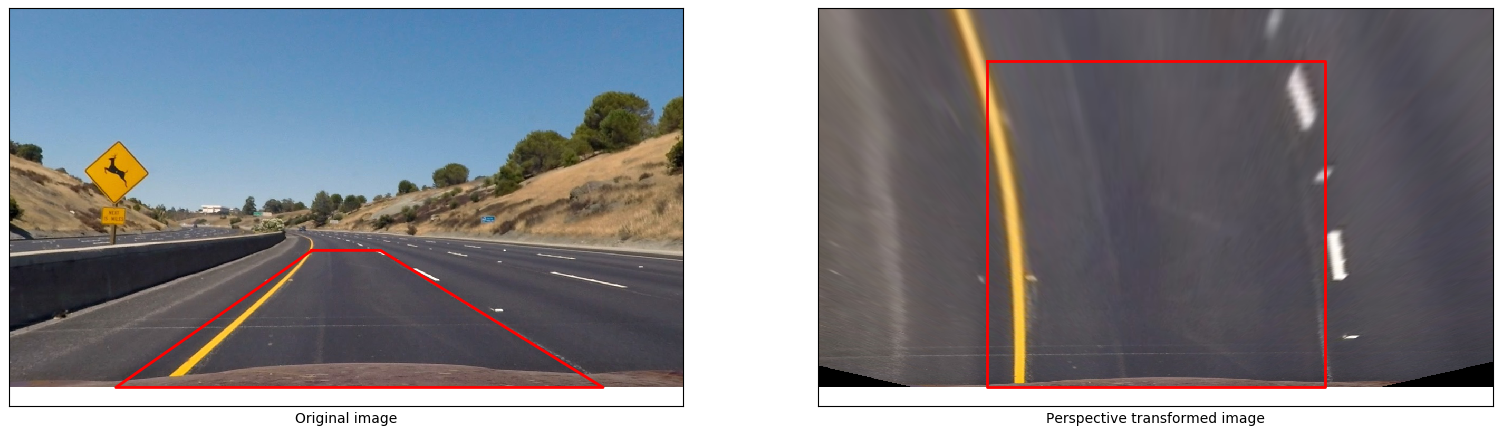
\includegraphics[width=\linewidth]{Figures/perspective_test2.png}}
            \caption{Final detected and tracked lanes}
            \end{figure}
            
            \begin{figure}[htbp]
            \centerline{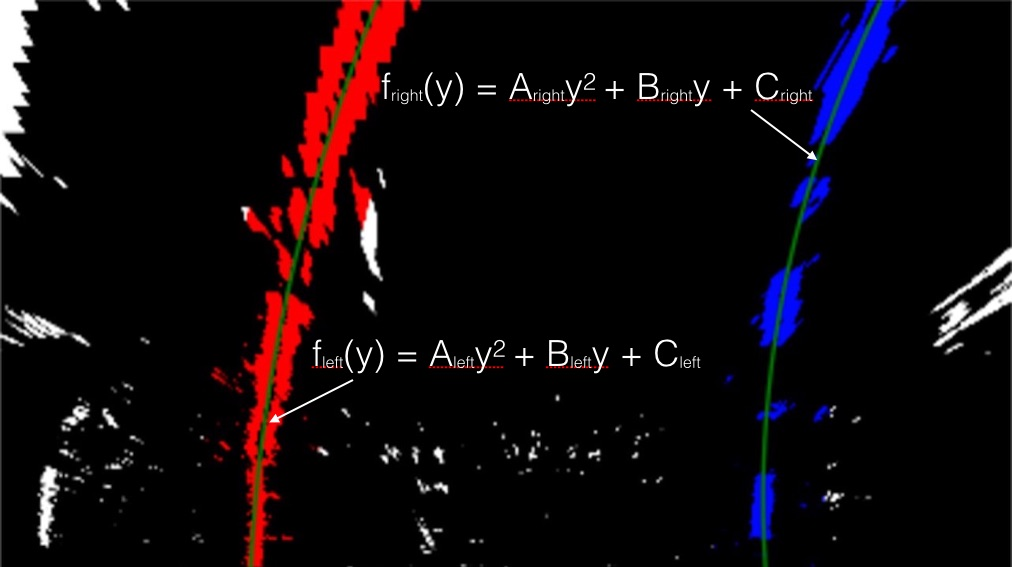
\includegraphics[width=\linewidth]{Figures/color_fit_lines.jpg}}
            \caption{Differentiating between left and right lanes}
            \end{figure}
    
            \begin{figure}[htbp]
            \centerline{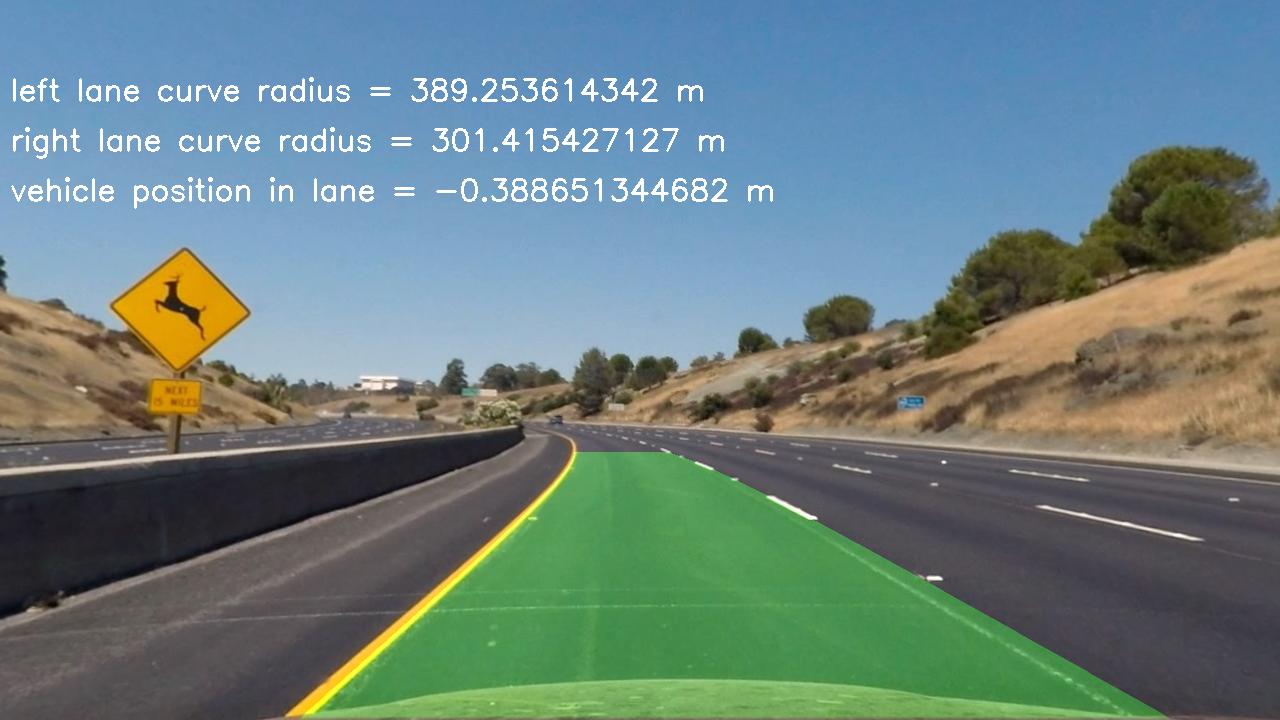
\includegraphics[width=\linewidth]{Figures/test2.jpg}}
            \caption{Final detected and tracked lanes}
            \end{figure}
            
    	\subsection{Driveable space segmentation}
    % 		\subsubsection{Data set exploration}
%         	{text\\}
    	\subsection{Object detection}
%     	{text\\}
    
  \section{Vehicle Control}
      \subsection{Vehicle Model}
      The Kinematic bicycle model of the vehicle is chosen, which unlike the dynamic model, ignores the vehicle's inertia and tire forces. The use of a dynamic model would be computationally expensive. Additionally, equations of tire models contain a term representing tire slip angle, which has the vehicle velocity in the denominator. Accordingly, in a situation where the vehicle comes to a stop, this term would cause computation errors, which prohibits generalization of the controller.
To derive the state transition equations of the model, a state vector should first be defined. The state vector is chosen to contain (\(x, y\)) to represent the position of the vehicle in the Cartesian space, \(\psi\) to represent its orientation, and (\(v\)) to represent its longitudinal velocity.
Actuated input allows the control of the vehicle state. Most cars have three inputs; the steering wheel, throttle pedal, and brake pedal. For simplicity, the brake and throttle controls are considered as a single acceleration control input (\(a\)), with the throttle represented as a positive value, and the brake as a negative value. Steering control is represented with \((\delta\)) as a value ranging from \(-1.0\) to \(1.0\).

\begin{equation}
x_{t+1}=x_{t}+v_t*cos(\psi_t)*dt
\label{st_x}
\end{equation}
\begin{equation}
y_{t+1}=y_{t}+v_t*sin(\psi_t)*dt
\label{st_y}
\end{equation}
The above equations \eqref{st_x} and \eqref{st_y} represent the state transition for the Cartesian coordinate of the vehicle, where (\(dt\)) is the time step length between samples states.
\begin{equation}
\psi_{t+1}=\psi_{t}+(v_t/L_f)*\delta_t*dt
\label{st_psi}
\end{equation}
The above equation \eqref{st_psi} represents the state transition equation for the vehicle orientation, where (\(L_f\)) is the distance between the center of mass of the vehicle and its front axle. The larger the vehicle, the slower the turn rate.
\begin{equation}
v_{t+1}=v_{t}+a_t*dt
\label{st_v}
\end{equation}
The above equation \eqref{st_v} represents the state transition equation for the vehicle longitudinal velocity.

      \subsection{PID controller}
      The PID controller is written in C++, and communicated with the simulator through a socket. At each time step, the simulator sends back data representing the current scene status. This includes the current vehicle state vector, and the track way points representing the center of the desired trajectory. Accordingly, the cross-track error (\(cte\)) is calculated and fed into the controller with a desired set point of \(0\) (to minimize \(cte\)).
\begin{figure}[htbp]
\centerline{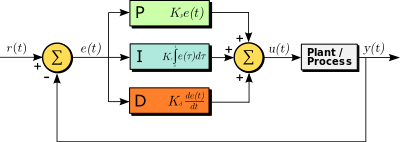
\includegraphics[width=\linewidth]{Figures/PID.png}}
\caption{PID control loop}
\end{figure}
\begin{itemize}
\item P (proportional) component is the most influential component on the behavior of the vehicle. It results in the counter-steer effect that is proportional and opposite to the \(cte\).
\item I (integral) component takes into account the integral of \(cte\) over the past time period. It corrects systematic bias and constant deviation which can prevent the controller from reaching the center of the reference trajectory, for example, if a zero steering angle does not map to a straight line steering.
\item D (differential) component is proportional to the rate of change of \(cte\), and is used to reduce oscillations and overshooting caused by the proportional component.
\end{itemize}
The vehicle state vector as well as the calculated error is recorded for a full lap around the track for later evaluation.

      \subsection{MPC controller}
      Given the centerline points of the road, the current vehicle state vector [\(x, y, \psi, v\)], and a state transition model (equations \eqref{st_x} - \eqref{st_v}), the controller predicts the optimal set of actuations that would minimize a weighted cost function over a finite time horizon. The vehicle model used is the kinematic bicycle model described above. For simplicity, all dynamic effects such as inertia, friction forces and torque are neglected. The model is non-linear due to the fact that it accounts for changes of heading direction.

The center trajectory is received from the simulator as a set of points, however, the reference trajectory is typically passed to the control block as a polynomial. A third order polynomial is chosen, since it will fit trajectories for most roads.

The two main error (cost) components to be minimized are the distance of the vehicle from the trajectory and the difference between vehicle orientation and trajectory orientation which are represented by the cross-track error \(cte\) and the orientation error \(e\psi\). The \(cte\) and \(e\psi\) are calculated and appended to the state vector. The resultant vector is be [\(x, y, \psi, v, cte, e\psi\)].

The \(cte\) of the successor state after time \(t\) is the state at \(t+1\). Accordingly, the state transition equation for \(cte\) is expressed as:
\begin{equation}
cte_{t+1} = cte_t + v_t* sin(e\psi_t) * dt
\label{st_cte_1}
\end{equation}

By linearizing the trajectory polynomial at the current vehicle position, \(f(x_t)\) is the reference line and the \(cte\) at the current state is defined as the difference between the linearized polynomial and the vehicle \(y\) position:
\begin{equation}
cte_t = y_t - f(x_t)
\label{cte}
\end{equation}
By substituting \eqref{cte} in \eqref{st_cte_1}:
\begin{equation}
cte_{t+1} = y_t - f(x_t) + v_t* sin(e\psi_t) * dt
\label{st_cte}
\end{equation}
Equation \eqref{st_cte} is broken down to two components:
\begin{itemize}
\item \(y_t - f(x_t)\) being the current \(cte\)
\item \(v_t* sin(e\psi_t) * dt\) being the change in \(cte\) caused by the vehicle's movement
\end{itemize}
Similarly, the state transition equation for the vehicle orientation error \(e\psi\) is represented as:
\begin{equation}
e\psi_{t+1} = e\psi_t + (v_t/L_f) * \delta_t * dt
\label{st_epsi_1}
\end{equation}
which is essentially the same as the state transition equation for the vehicle orientation (\(\psi\)) in equation \eqref{st_psi}.
The vehicle orientation error \(e\psi\) is the difference between the current vehicle orientation and the desired (reference) orientation.
\begin{equation}
e\psi_t = \psi_t - \psi^{ref}_t
\label{epsi}
\end{equation}
where \(\psi_t\) is the vehicle orientation from the state vector, and \(\psi^{ref}_t\) is the desired orientation, which is calculated as the tangential angle of the polynomial \(f\) evaluated at \(x_t\) as \(\arctan(f'(x_t))\), where \(f'\) is the derivative of the polynomial. The final state transition equation for the error in orientation is derived by substituting equation \eqref{epsi} in \eqref{st_epsi_1}
\begin{equation}
e\psi_{t+1} = \psi_t - \psi^{ref}_t + (v_t/L_f) * \delta_t * dt
\label{st_epsi}
\end{equation}
Similarly to the cross-track error this is broken down to two components:
\begin{itemize}
\item \(\psi_t - \psi^{ref}_t\) being current orientation error.
\item \((v_t/L_f) * \delta_t * dt\) being the change in orientation error caused by the vehicle's movement.
\end{itemize}

Ideally, a cost function with \(cte\) and \(e\psi\) as its only components would guarantee that there would be no difference between the actual vehicle position and heading, and the desired position and heading. However, several errors might occur with such simple cost function. For example, the vehicle might stop in a situation where any further actuation would increase the cost, in addition to erratic behavior due to the drastically different consecutive actuations. To solve such issues, other components are added to the cost functions. The solution to the problem of stopping is the addition of a term representing the difference between the current velocity and a reference velocity value which increases the cost function whenever velocity falls below the reference value. Other terms are added to penalize large steering angles, high velocity turns, and high fluctuations of the steering angle.

The prediction horizon is the duration over which future predictions are made, referred to as \(T\), which is the product of two other variables, \(N\) and \(dt\), representing the number of time steps in the horizon, and the time duration between actuations respectively. The goal of controller is to optimize the control inputs: \([\delta, a]\). An optimizer \cite{ipopt} used to tune these inputs to find a low cost vector of control inputs with the length equal to \(N\). Accordingly, \(N\) determines the number of variables optimized by the controller, and this the computational cost. As the value of \(dt\) increases, the frequency of actuations decreases, which in turn decreases the approximation accuracy of a continuous reference trajectory, which is referred to as "discretization error". For the specific application of autonomous driving in the Udacity simulator, \(N\) is chosen as \(10\), and \(dt\) is chosen as \(0.1 sec\). The code for the MPC is written in c++ as well.

The controller is able to successfully complete several laps around the simulator track at speeds as high as \(100 mph\).


\chapter{Behavioral Reflex Approach (End-to-End)}
	\section{Imitation Learning}
        % \subsection{Nvidia PilotNet}
        % \subsection{Human Driver Behavior Imitation}
       	\subsection{MPC Behavior Imitation}
        The main goal is to train an End-to-End Artificial Deep Neural Network to successfully drive a vehicle in the simulator using only the front-camera raw data as an input. Imitation learning is the algorithm used to train such network. The basic idea behind imitation learning is to train a controller that mimics an expert's demonstration. The assumption is that the expert is successful at performing the task of interest and that a controller trained to mimic the expert will also perform the task well.

Since the MPC is successful at completing several laps around the simulator track, it is used as the expert during data collection. The MPC is allowed to drive the vehicle around the track with a reference velocity of \(30 mph\). At each time step, the image received from the camera, as well as the steering angle command produced by the controller are recorded. About 35,000 frames are collected.

The implemented network is a Deep Convolution Neural Network (CNN) based on the Nvidia PilotNet architecture\cite{nvidia}. The model is implemented using \(Keras\), running with \(tensorflow\) as the backend. The network contains an input image normalization layer, 5 convolution layers, and 4 fully connected layers, the final layer is responsible of the final steering output.

Since the majority of the track is almost straight, training data has to be filtered to remove any bias towards producing a \(0\) steering angle. The resultant data contained 14,500 frames which are then divided into a training set and validation set with the ratio \(80:20\) respectively. Camera frames will cropped to focus only on the road ahead. This prevents confusion from irrelevant features that should not contribute to the driving action such as the sky and trees. The network is trained for \(35\) epochs, with a batch size of \(64\). The Adam optimizer is used \cite{adam} and a learning rate of \(0.0001\) is found to yield the best performance. The network is able to complete several laps around track as well.
    %     \subsection{Real Urban data testing}
    % \section{Conditional Imitation Learning}
    %     {text\\}
    %     \subsection{Data Exploration and Augmentation}
    %     {text\\}


    